\documentclass[article]{jss}
\usepackage{lmodern}
\usepackage{amssymb,amsmath}
\usepackage{ifxetex,ifluatex}
\usepackage{fixltx2e} % provides \textsubscript
\ifnum 0\ifxetex 1\fi\ifluatex 1\fi=0 % if pdftex
  \usepackage[T1]{fontenc}
  \usepackage[utf8]{inputenc}
\else % if luatex or xelatex
  \ifxetex
    \usepackage{mathspec}
    \usepackage{xltxtra,xunicode}
  \else
    \usepackage{fontspec}
  \fi
  \defaultfontfeatures{Mapping=tex-text,Scale=MatchLowercase}
  \newcommand{\euro}{€}
\fi
% use upquote if available, for straight quotes in verbatim environments
\IfFileExists{upquote.sty}{\usepackage{upquote}}{}
% use microtype if available
\IfFileExists{microtype.sty}{%
\usepackage{microtype}
\UseMicrotypeSet[protrusion]{basicmath} % disable protrusion for tt fonts
}{}
\usepackage{color}
\usepackage{fancyvrb}
\newcommand{\VerbBar}{|}
\newcommand{\VERB}{\Verb[commandchars=\\\{\}]}
\DefineVerbatimEnvironment{Highlighting}{Verbatim}{commandchars=\\\{\}}
% Add ',fontsize=\small' for more characters per line
\usepackage{framed}
\definecolor{shadecolor}{RGB}{248,248,248}
\newenvironment{Shaded}{\begin{snugshade}}{\end{snugshade}}
\newcommand{\AlertTok}[1]{\textcolor[rgb]{0.94,0.16,0.16}{#1}}
\newcommand{\AnnotationTok}[1]{\textcolor[rgb]{0.56,0.35,0.01}{\textbf{\textit{#1}}}}
\newcommand{\AttributeTok}[1]{\textcolor[rgb]{0.77,0.63,0.00}{#1}}
\newcommand{\BaseNTok}[1]{\textcolor[rgb]{0.00,0.00,0.81}{#1}}
\newcommand{\BuiltInTok}[1]{#1}
\newcommand{\CharTok}[1]{\textcolor[rgb]{0.31,0.60,0.02}{#1}}
\newcommand{\CommentTok}[1]{\textcolor[rgb]{0.56,0.35,0.01}{\textit{#1}}}
\newcommand{\CommentVarTok}[1]{\textcolor[rgb]{0.56,0.35,0.01}{\textbf{\textit{#1}}}}
\newcommand{\ConstantTok}[1]{\textcolor[rgb]{0.00,0.00,0.00}{#1}}
\newcommand{\ControlFlowTok}[1]{\textcolor[rgb]{0.13,0.29,0.53}{\textbf{#1}}}
\newcommand{\DataTypeTok}[1]{\textcolor[rgb]{0.13,0.29,0.53}{#1}}
\newcommand{\DecValTok}[1]{\textcolor[rgb]{0.00,0.00,0.81}{#1}}
\newcommand{\DocumentationTok}[1]{\textcolor[rgb]{0.56,0.35,0.01}{\textbf{\textit{#1}}}}
\newcommand{\ErrorTok}[1]{\textcolor[rgb]{0.64,0.00,0.00}{\textbf{#1}}}
\newcommand{\ExtensionTok}[1]{#1}
\newcommand{\FloatTok}[1]{\textcolor[rgb]{0.00,0.00,0.81}{#1}}
\newcommand{\FunctionTok}[1]{\textcolor[rgb]{0.00,0.00,0.00}{#1}}
\newcommand{\ImportTok}[1]{#1}
\newcommand{\InformationTok}[1]{\textcolor[rgb]{0.56,0.35,0.01}{\textbf{\textit{#1}}}}
\newcommand{\KeywordTok}[1]{\textcolor[rgb]{0.13,0.29,0.53}{\textbf{#1}}}
\newcommand{\NormalTok}[1]{#1}
\newcommand{\OperatorTok}[1]{\textcolor[rgb]{0.81,0.36,0.00}{\textbf{#1}}}
\newcommand{\OtherTok}[1]{\textcolor[rgb]{0.56,0.35,0.01}{#1}}
\newcommand{\PreprocessorTok}[1]{\textcolor[rgb]{0.56,0.35,0.01}{\textit{#1}}}
\newcommand{\RegionMarkerTok}[1]{#1}
\newcommand{\SpecialCharTok}[1]{\textcolor[rgb]{0.00,0.00,0.00}{#1}}
\newcommand{\SpecialStringTok}[1]{\textcolor[rgb]{0.31,0.60,0.02}{#1}}
\newcommand{\StringTok}[1]{\textcolor[rgb]{0.31,0.60,0.02}{#1}}
\newcommand{\VariableTok}[1]{\textcolor[rgb]{0.00,0.00,0.00}{#1}}
\newcommand{\VerbatimStringTok}[1]{\textcolor[rgb]{0.31,0.60,0.02}{#1}}
\newcommand{\WarningTok}[1]{\textcolor[rgb]{0.56,0.35,0.01}{\textbf{\textit{#1}}}}
\usepackage{longtable,booktabs}
% \ifxetex
%   \usepackage[setpagesize=false, % page size defined by xetex
%               unicode=false, % unicode breaks when used with xetex
%               xetex]{hyperref}
% \else
%   \usepackage{hyperref}
% \fi
% \hypersetup{breaklinks=true,
%             bookmarks=true,
%             pdfauthor={},
%             pdftitle={},
%             colorlinks=true,
%             citecolor=blue,
%             urlcolor=blue,
%             linkcolor=magenta,
%             pdfborder={0 0 0}}
\urlstyle{same}  % don't use monospace font for urls
\setlength{\parindent}{0pt}
\setlength{\parskip}{6pt plus 2pt minus 1pt}
\setlength{\emergencystretch}{3em}  % prevent overfull lines
\setcounter{secnumdepth}{5}

%%% Use protect on footnotes to avoid problems with footnotes in titles
\let\rmarkdownfootnote\footnote%
\def\footnote{\protect\rmarkdownfootnote}

%%% need tightlist which is included in pandoc header
\providecommand{\tightlist}{%
  \setlength{\itemsep}{0pt}\setlength{\parskip}{0pt}}
  
\newlength{\cslhangindent}
\setlength{\cslhangindent}{1.5em}
\newlength{\csllabelwidth}
\setlength{\csllabelwidth}{3em}
\newenvironment{CSLReferences}[2] % #1 hanging-ident, #2 entry spacing
 {% don't indent paragraphs
  \setlength{\parindent}{0pt}
  % turn on hanging indent if param 1 is 1
  \ifodd #1 \everypar{\setlength{\hangindent}{\cslhangindent}}\ignorespaces\fi
  % set entry spacing
  \ifnum #2 > 0
  \setlength{\parskip}{#2\baselineskip}
  \fi
 }%
 {}
\usepackage{calc}
\newcommand{\CSLBlock}[1]{#1\hfill\break}
\newcommand{\CSLLeftMargin}[1]{\parbox[t]{\csllabelwidth}{#1}}
\newcommand{\CSLRightInline}[1]{\parbox[t]{\linewidth - \csllabelwidth}{#1}\break}
\newcommand{\CSLIndent}[1]{\hspace{\cslhangindent}#1}


\author{
Shimeng Huang\\University of Waterloo \And Martin Lysy\\University of Waterloo
}
\title{\pkg{flexEL}: A Fast and Flexible Framework for Empirical Likelihood Modeling}

\Plainauthor{Shimeng Huang, Martin Lysy}
\Plaintitle{flexEL: A Fast and Flexible Framework for Empirical Likelihood Modeling}

\Abstract{
This paper introduces \pkg{flexEL}, a fast and flexible framework for implementing and calibrating empirical likelihood models. In particular, it provides the loglikelihood and gradient functions for arbitrary moment constraint matrices. The inner optimization problem is efficiently computed in C++ using the ``Eigen'' linear algebra library. The package also provides functions for implementing right-censored regression models, where the inner optimization is conducted via an expectation-maximation algirithm. Users may interface with the library through \proglang{R} or directly through C++, as the underlying C++ code is exposes as a standalone header-only library.
}

\Keywords{empirical likelihood, quantile regression, EM algorithm, right-censoring, location-scale model, \proglang{R}}
\Plainkeywords{empirical likelihood, quantile regression, EM algorithm, right-censoring, location-scale model, R}

%% publication information
%% \Volume{50}
%% \Issue{9}
%% \Month{June}
%% \Year{2012}
%% \Submitdate{}
%% \Acceptdate{2012-06-04}

\Address{
      Martin Lysy\\
  University of Waterloo\\
  200 University Avenue West\\Ontario, Canada\\
  E-mail: \email{mlysy@uwaterloo.ca}\\
  
  }

% %   \title{true}
%   % % % %   \author{true \\ true}
%   % % %   %   \date{2021-11-07}
% 
\usepackage{caption}
\captionsetup[table]{skip=.1em}
\usepackage{bm}
\usepackage{amsmath}
\newcommand{\s}{\sigma}
\newcommand{\XX}{\bm X}
\newcommand{\xx}{\bm x}
\newcommand{\yy}{\bm y}
\newcommand{\zz}{\bm z}
\newcommand{\uu}{\bm u}
\newcommand{\qq}{\bm q}
\newcommand{\ee}{\bm e}
\newcommand{\tth}{\bm \theta}
\newcommand{\lla}{\bm \lambda}
\newcommand{\bbe}{\bm \beta}
\newcommand{\gga}{\bm \gamma}
\newcommand{\eep}{\bm \epsilon}
\newcommand{\oom}{\bm \omega}
\newcommand{\R}{\mathbb R}
\renewcommand{\gg}{\bm g}
\newcommand{\w}{\omega}
\renewcommand{\l}{\lambda}
\newcommand{\g}{\gamma}
\renewcommand{\L}{\mathcal{L}}
\renewcommand{\E}{\textrm{E}}
\newcommand{\EL}{\textrm{EL}}
\newcommand{\CEL}{\textrm{CEL}}
\newcommand{\SCEL}{\textrm{SCEL}}
\newcommand{\str}[1]{{#1}^{\star}}
\DeclareMathOperator*{\argmax}{arg\,max}
\DeclareMathOperator*{\argmin}{arg\,min}
\newcommand{\e}{\varepsilon}
\newcommand{\iid}{\stackrel {\textrm{iid}}{\sim}}
\renewcommand{\|}{\,|\,}
\newcommand{\sha}[1]{{#1}^{\sharp}}
\newcommand{\ud}{\mathop{}\!\mathrm{d}}
\newcommand{\dth}{\frac{\ud}{\ud\tth}}

\begin{document}

\maketitle

% % \begin{abstract}
% This paper introduces \pkg{flexEL}, a fast and flexible framework for implementing and calibrating empirical likelihood models. In particular, it provides the loglikelihood and gradient functions for arbitrary moment constraint matrices. The inner optimization problem is efficiently computed in C++ using the ``Eigen'' linear algebra library. The package also provides functions for implementing right-censored regression models, where the inner optimization is conducted via an expectation-maximation algirithm. Users may interface with the library through \proglang{R} or directly through C++, as the underlying C++ code is exposes as a standalone header-only library.
% \end{abstract}
% 
\hypertarget{introduction}{%
\section{Introduction}\label{introduction}}

Empirical likelihood (EL) method allows statisticians to construct partially specified models via moment conditions. Although an EL model does not assume any parametric family of the data, the estimator is in some sense as efficient as a fully parametric model (Qin and Lawless 1994).

The empirical likelihood (EL) approach can be traced back to Thomas and Grunkemeier (1975). Its current framework is mainly developed by Owen (1988), Owen (1990), and Owen (1991), where empirical likelihood ratio statistics is introduced, and the EL method is extended to linear regression models under fixed or random design. Kolaczyk (1994) further generalize the method to be used with generalized linear models. Qin and Lawless (1994) relate estimating equation and empirical likelihood and provide asymptotic properties of the estimator. J. Chen, Variyath, and Abraham (2008) propose an adjustment to the constraints in the EL framework to ensure the convex hall condition is always satisfied and the theoretical properties are not affected. Moreover, Lazar (2003) explores the validity of using empirical likelihood for Bayesian inference as well as the frequentist properties of the posterior intervals. Chaudhuri, Mondal, and Yin (2017) considers using Hamiltonian Monte Carlo sampling for the Bayesian EL models.

An approach related to EL is the so-called exponentially tilting (ET) method (Efron 1981). Schennach (2005), and Schennach (2007) propose the exponentially tilted empirical likelihood (ELET) approach, which enjoys the properties of both ET and EL methods. Newey and Smith (2004) also gives the theoretical results relating Generalized Method of Moment (GMM) and Generalized Empirical Likelihood (GEL), their higher order properties, as well as their bias-corrected forms in the absence of length-bias.

For EL with length-biased data, Zhou (2005) proposes an EM algorithm for censored and truncated data under mean type constraints without covariates. Zhou and Li (2008) combine the empirical likelihood with the Buckley-James estimator which works for regression models. Zhou, Kim, and Bathke (2012) revisit the fixed and random design linear regression models but for right-censored data and show that the model works well even with heteroscedastic errors. Shen, Yuen, and Liu (2016) develop a different EM algorithm under the EL framework for one- or two- sample doubly censored data.

Given fully observed data, an asymptotic \(\chi^2\) distribution of log EL is valid. When right-censoring is present, the asymptotic distribution is no longer a standard \(\chi^2\) distribution but subject to an unknown scaling factor. He et al. (2016) consider using a special influence functions in the estimating equations to retain a standard \(\chi^2\) distribution. Li and Wang (2003) propose an adjusted EL for linear regression using synthetic data approach. Ning et al. (2013) consider length-biased right-censored data in a non-regression setting for the estimation of mean, quantile and survival function of the population as well as confidence intervals.

Although the EL method has been extended and generalized over the years, there has not been a flexible and efficient software available to the public. The existing software are either written in a high-level programming language for which inner optimization is not efficient, or are designed for specific regression problems (e.g.~\pkg{emplik}, \pkg{gelS4}). There is also no software that provides EL method for right-censored data.

This paper describes a framework we designed for EL researchers to develop fast and efficient implementations of their own EL models and related methods. We provide a computationally efficient R package called \pkg{flexEL} which is flexible enough for users to solve any type of regression problems with minimum programming effort. The computational efficiency is achieved by a C++ implementation of the Newton--Raphson algorithm which is a key step in the EL inner optimization problem. Other than the main functionality of regular EL estimation, the package also provides support correction, continuity correction under right-censoring, gradient calculation, as well as various mean and quantile regression models for which the details will be described in the later sections.

\hypertarget{methodology}{%
\section{Methodology}\label{methodology}}

\hypertarget{basics}{%
\subsection{Basics}\label{basics}}

Let \(\bm X= (\bm x_1,\cdots,\bm x_n)\) where \(\bm x_i\in\mathbb R^d\) be iid observations from an unknown distribution \(F_0(\bm x)\), about which a parameter of interest \(\bm \theta\in \mathbb R^p\) is defined as satisfying an \(m\)-dimensional moment condition:
\begin{equation} \label{eq:momcond}
  \textrm{E}\bigl[\bm g(\bm x;\bm \theta)\bigr] = 0,
\end{equation}
where \(\bm g(\bm x, \bm \theta) = \bigl( g_1(\bm x, \bm \theta), \ldots, g_m(\bm x, \bm \theta) \bigr)\).

The empirical likelihood \(\textrm{EL}(\bm \theta)\) as the profile likelihood over the distribution function of \(\bm x\):
\begin{equation} \label{eq:elF}
  \textrm{EL}(\bm \theta) = \max_{F \in \mathcal F(\bm \theta)} \prod_{i=1}^n \mathrm{d} F(\bm x_i),
\end{equation}
where for any given \(\bm \theta\), \(\mathcal F(\bm \theta)\) is the set of (valid) distribution functions satisfying \eqref{eq:momcond}.

For any \(\bm \theta\), Owen (1988) has shown that the maximum of \eqref{eq:elF} can be achieved by focusing on the distribution functions having all mass on the support of the observed data \(\bm x_1, \cdots, \bm x_n\), and the infinite-dimensional profile likelihood \eqref{eq:elF} can be reduced to a finite-dimensional one.

To have a general notation consistent with the EM algorithm under right-censoring in later sections, we now define \textbf{weighted empirical likelihood}:

\begin{equation}
  \textrm{EL}(\bm \theta) = \prod_{i=1}^n \hat{\omega_i}(\bm \theta)^{q_i},
\end{equation}

where \(q_i > 0, \forall i=1,\cdots,n\), and the \(n\)-dimensional vector of probability weights \(\hat{\omega}(\bm \theta)\) associated with the observations is the solution of an inner optimization problem which will be referred to as \textbf{EL inner optimization}:

\begin{equation} \label{eq:noncensopt}
\begin{split}
  \max_{\omega}\quad & \sum_{i=1}^n q_i \log(\omega_i) \\
  \text{s.t.}\quad & \sum_{i=1}^n \omega_i\cdot g(\bm x_i;\bm \theta) = 0 \\
  & \sum_{i=1}^n \omega_i = 1 \\
  & \omega_i \geq 0, \quad i=1,\cdots,n.
\end{split}
\end{equation}

When \(q_i = 1, \forall i=1,\cdots,n\), we have the regular empirical likelihood function. The problem in (\ref{eq:noncensopt}) is a constrained convex optimization problem, and its optimal solution can be found via Lagrangian function, similar to the steps in Owen (1990). Specifically, the Lagrangian function can be set up as
\begin{equation} \label{eq:lagrange}
  \mathcal{L}= \sum_{i=1}^n q_i\log(\omega_i) + (\sum_{i=1}^n q_i)\bm \lambda'(\sum_{i=1}^n \omega_i \cdot g(\bm x_i;\bm \theta)) + \mu(1-\sum_{i=1}^n \omega_i).
\end{equation}

Let \(r_i = q_i/\sum_{i=1}^n q_i\). Provided that \(\bm 0\) is in the convex full of the points \(g(\bm x_i;\bm \theta),\cdots,g(\bm x_n;\bm \theta)\), a unique optimal probability vector exist and can be shown to be

\begin{equation}\label{eq:omegahat}
  \hat{\omega_i}(\bm \theta) = \frac{r_i}{1 - \hat{\bm \lambda}'(\bm \theta) g(\bm x_i;\bm \theta)},
\end{equation}

where

\begin{equation}
\begin{aligned}
\hat{\bm \lambda}(\bm \theta) &= \mathop{\mathrm{arg\,max}}_{\bm \lambda(\bm \theta)} \sum_{i=1}^n r_i\ {\log}^{\star}\left(1 - \bm \lambda'(\bm \theta) g(\bm x_i;\bm \theta); r_i\right), \\
{\log}^{\star}(x; r) &= 
\begin{cases} 
\log(x) & x \ge r \\
- \frac{1}{2} (x/r)^2 + 2 (x/r) - \frac{3}{2} + \log r & x < r.
\end{cases}
\end{aligned}
\label{eq:optim}
\end{equation}

Qin and Lawless (1994) has shown that \(\bm \lambda(\bm \theta)\) is a continuous differentiable function of \(\bm \theta\) provided that convex hull condition is satisfied with \(\bm \theta\) and \(\sum_{i=1}^n g(\bm x_i;\bm \theta)g'(\bm x_i;\bm \theta)\) is positive definite. However, the support of \(\bm \theta\) is not necessarily a convex set, as demonstrated by Chaudhuri, Mondal, and Yin (2017).

In the case that we are only interested in one parameter \(\theta\) of an unknown distribution \(F\), Owen (1990) has shown that the limiting distribution of the EL ratio statistic is chi-square. For a vector of parameters, Qin and Lawless (1994) shows that the EL ratio statistic is asymptotic normal. This means that we can derive confidence intervals of the parameters accordingly.

With the Lagrangian function in (\ref{eq:lagrange}), we can also derive the gradient of \(\mathcal{L}\) with respect to \(\bm \theta\), which allows one to employ a gradient based optimization algorithm to find the optimal solution of the estimator. Specifically, the gradient of the the weighted empirical log likelihood with respect to \(\bm \theta\) can be derived as

\begin{equation}
\frac{\mathop{}\!\mathrm{d}}{\mathop{}\!\mathrm{d}\bm \theta}\log \textrm{EL}(\bm \theta) = Q \sum_{i=1}^n \hat \omega_i(\bm \theta) \cdot \bm \lambda(\bm \theta)' \frac{\mathop{}\!\mathrm{d}}{\mathop{}\!\mathrm{d}\bm \theta}g_i(\bm \theta),
\end{equation}

where \(Q = \sum_{i=1}^n q_i\).

\hypertarget{support-correction}{%
\subsection{Support Correction}\label{support-correction}}

Let \(g_i = g(\bm x_i;\bm \theta)\) for \(i = 1,\cdots, n\). As mentioned above, a necessary condition of obtaining a unique optimal solution is that \(\bm 0\) is in the convex full of the points \(g_1,\cdots,g_n\) which may not be satisfied with the data. J. Chen, Variyath, and Abraham (2008) propose a method to handle this situation by adding one more constraint in the EL inner optimization problem (\ref{eq:noncensopt}), that is

\begin{equation} \label{eq:noncensoptadj}
\begin{split}
  \max_{\omega}\quad & \sum_{i=1}^{n+1} q_i \log(\omega_i) \\
  \text{s.t.}\quad & \sum_{i=1}^{n+1} \omega_i\cdot g_i = 0 \\
  & \sum_{i=1}^{n+1} \omega_i = 1 \\
  & \omega_i \geq 0, \quad i=1,\cdots,{n+1},
\end{split}
\end{equation}

where \(g_{n+1} = -\frac{a_n}{n} \sum_{i=1}^n g_i\) for some small positive \(a_n\).

It is also shown by J. Chen, Variyath, and Abraham (2008) that this approach retains the optimally properties of EL, is faster to compute, and improves coverage probabilities of the confidence regions.

\hypertarget{regression-with-right-censored-outcome}{%
\subsection{Regression with Right-Censored Outcome}\label{regression-with-right-censored-outcome}}

\hypertarget{empirical-likelihood-with-right-censored-outcome-variable}{%
\subsubsection{Empirical Likelihood with Right-Censored Outcome Variable}\label{empirical-likelihood-with-right-censored-outcome-variable}}

\pkg{flexEL} handles the situation of regression models with right-censored outcomes, that is, instead of observing outcomes \(y_i\), we observe \(u_i = \min(y_i, c_i)\) and \(\delta_i = \mathfrak 1\{y_i \le c_i\}\), where \(c_i\) is the censoring time.

Consider a general regression model
\[
  y_i = f(\bm x_i; \bm \theta) + \varepsilon_i, \quad i=1,\cdots,n
\]
where \(\varepsilon_i\) follows an unknown distribution with mean \(0\) and variance \(1\), and independent of \(\bm x_i\), and \(m\)-dimensional conditional moment restrictions
\begin{equation}\label{eq:cmom}
  \textrm{E}\bigl[\bm g(\bm x, \varepsilon; \bm \theta) \,|\, \bm x\bigr] = 0.
\end{equation}

We assume that the censoring variable \(c_i\) independent of \(y_i\). Let's denote the residuals given a specific \(\bm \theta\) as \(e_i'\)s (corresponding to \(u_i'\)s), the complete residuals as \(\varepsilon_i'\)s (corresponding to \(y_i'\)s).

The empirical likelihood with censored observations once again is defined by profiling over the unknown joint distribution function \(F(\bm x,\varepsilon) = G(\bm x) \cdot H(\varepsilon)\), where \(G\) and \(H\) are the CDFs of \(\bm x\) and \(\varepsilon\):
\begin{equation}\label{eq:celF}
  \textrm{CEL}(\bm \theta) = \max_{F \in \mathcal F(\bm \theta)}\prod_{i=1}^n dG(\bm x_i) \cdot dH(\varepsilon_i)^{\delta_i} \cdot [1- H(e_i)]^{1-\delta_i},
\end{equation}
where
\[
  e_i = e_i(\bm \theta) = \frac{u_i - \mu(\bm x_i;\bm \theta)}{\eta(\bm x_i;\bm \theta)},
\]
and \(\mathcal F(\bm \theta)\) is the set of all valid distribution functions satisfying \eqref{eq:cmom}. It is not hard to show that for any choice of \(H(\varepsilon)\), the maximum of \eqref{eq:celF} over \(G(\bm x)\) is attained as the empirical distribution \(\hat G(\bm x)\) which puts a point mass of \(1/n\) on each covariate observation \(\bm x_1, \ldots, \bm x_n\). Restricting our attention to \(G(\bm x)\) uniform on the observed covariates, and considering only the weaker moment condition
\begin{equation}\label{eq:umom}
  \textrm{E}\bigl[\bm g(\bm x, \varepsilon; \bm \theta)\bigr] = 0
\end{equation}
(which is true for any \(G(\bm x)\) if \eqref{eq:cmom} holds), the CEL function reduces to
\[
  \textrm{CEL}(\bm \theta) = \max_{F \in \mathcal F^\star(\bm \theta)}\prod_{i=1}^n dH(e_i)^{\delta_i} \cdot [1- H(e_i)]^{1-\delta_i},
\]
where \(\mathcal F^\star(\bm \theta)\) is the set of all valid distributions \(F(\bm x, \varepsilon)\) satisfying \eqref{eq:umom}.

It can be shown that with censored observations, it is no longer true that an optimal \(F\) has support only on the data points \(e_i, i=1,\cdots,n\). However, if we restrict ourselves to this case, we arrive at a finite dimensional problem
\begin{equation} \label{eq:elcens}
  \textrm{CEL}(\bm \theta) = \prod_{i=1}^n \Big[\hat \omega_i(\bm \theta)^{\delta_i}(\sum_{j: e_j \geq e_i}\hat \omega_i(\bm \theta))^{1-\delta_i}\Big].
\end{equation}

where similar as before, \(\hat\omega(\bm \theta)\) is the solution of an inner optimization problem

\begin{equation} \label{eq:elcens_inner}
\begin{split}
  \max_{\omega}\quad & \sum_{i=1}^n \Big[\delta_i\log(\omega_i) + (1-\delta_i)\log(\sum_{j: e_j\geq e_i}\omega_i)\Big]\\
  \text{s.t.}\quad & \sum_{i=1}^n \omega_i\cdot g_i(\bm y,\bm x;\bm \theta) = 0 \\
  & \sum_{i=1}^n \omega_i = 1 \\
  & \omega_i \geq 0, \quad i=1\cdots,n.
\end{split}
\end{equation}

Right-censoring is essentially a missing data problem. In \pkg{flexEL}, the right-censored EL problem is solved via an EM algorithm. The algorithm is a generalization of Zhou (2005) to regression problems.

\hypertarget{an-em-algorithm}{%
\subsubsection{An EM Algorithm}\label{an-em-algorithm}}

Recall that if \(\delta_i=1\), we have \(e_i=\varepsilon_i\). This means that the \textbf{unobserved (latent) variables} are the \(\varepsilon_i'\)s such that \(\delta_i = 0\), the \textbf{complete data likelihood} is
\begin{equation}\label{eq:complike}
  \ell(\omega,\varepsilon|\bm u) = \sum_{i=1}^n\log(\prod_{j=1}^n \omega_j^{\mathfrak 1(\varepsilon_i=e_j)})
\end{equation}

The E-step of the EM algorithm takes the expectation of (\ref{eq:complike}) with respect to \(\bm y\) (vector of all latent variables) conditioned on the observed values, the censoring indicator and the current state of the parameters, and since for \(\delta_i = 1\), we know that \(u_i=y_i\), we have

\begin{equation}\label{eq:estep}
\begin{split}
  \textrm{E}_{\varepsilon|e,\delta,\omega_0}\bigl[\ell(\omega,\varepsilon|e)\bigr]
  &= \textrm{E}_{\varepsilon|e,\delta,\omega_0}\Bigl[\sum_{i=1}^n\delta_i\log(\omega_i) +
  (1-\delta_i)\log(\prod_{j=1}^n \omega_j^{\mathfrak 1(\varepsilon_i=e_j)})\Bigr] \\
  &= \sum_{i=1}^n\Bigl[\delta_i\log(\omega_i) +
  (1-\delta_i)\sum_{j=1}^n \textrm{E}_{\varepsilon_i|e,\delta,\omega_0}[\mathfrak1(\varepsilon_i=e_j)]\log(\omega_j)\Bigr] \\
  &= \sum_{i=1}^n\Bigl[\delta_i\log(\omega_i) +
  (1-\delta_i)\sum_{j=1}^n P_{\varepsilon_i|e,\delta,\omega_0}(\varepsilon_i=e_j)\log(\omega_j)\Bigr].
\end{split}
\end{equation}

Notice that we can write
\[
  \log(\prod_{j=1}^n \omega_j^{\mathfrak 1(\varepsilon_i=e_j)}) =
  \sum_{i=1}^n \mathfrak 1(\varepsilon_i=e_j)\log(\omega_j),
\]
because for any \(i \in \{1,\cdots,n\}\), \(\mathfrak 1(\varepsilon_i=e_j)=1\) for one and only one \(j\in\{1,\cdots,n\}\). Also, the latent \(\varepsilon_i's\) are independent but not identically distributed, since each of them follows a different categorical distribution (multinomial distribution with one trial).

The conditional distribution in (\ref{eq:condprob_orig}) is a categorical distribution conditioned on that the probability mass only allocates on the values in a subset of \(\{e_1,\cdots,e_n\}\) such that \(\mathfrak 1(e_j\geq e_i) = 1\) for \(j=1,\cdots,n\), which is still a multinomial distribution.
\begin{equation}\label{eq:condprob_orig}
  P_{\varepsilon_i|e,\delta,\omega_0}(\varepsilon_i=e_j) =
  \frac{\mathfrak 1(e_j\geq e_i)\cdot \omega_{0j}}{\sum_{k=1}^n\mathfrak 1(e_k\geq e_i)\cdot\omega_{0k}}.
\end{equation}

Therefore, the EM algorithm iterates between the following two steps:

\begin{itemize}
\item \textbf{E-step:} Given the observed values and the weights $\omega_0$ from the previous iteration, the expectation of the log likelihood is
\begin{equation}\label{eq:emestep}
\begin{split}
  \textrm{E}_{\varepsilon|e,\delta,\omega_0}[\ell(\omega,\varepsilon|e)]
  &= \sum_{i=1}^n \Big[\delta_i \log \omega_i +
    (1-\delta_i) \sum_{j: e_j\geq e_i} \tilde \omega_{ij} \log \omega_j\Big] \\
  &= \sum_{i=1}^n \Big[\delta_i + \sum_{k: e_k\leq e_i} (1-\delta_k)
      \cdot\tilde\omega_{ki}\Big]\cdot\log \omega_i,
\end{split}
\end{equation}
where
\[
  \tilde \omega_{ki} = \frac{\omega_{0i}}{\sum_{l: e_l\geq e_k}\omega_{0l}}, \quad k,i: e_k\leq e_i.
\]

\item \textbf{M-step:}
Let $q_i = \delta_i + \sum_{k: e_k\leq e_i} (1-\delta_k)\cdot \tilde \omega_{ki}$ for $i=1,\cdots,n$, then the problem becomes
\begin{equation}\label{eq:emmstep}
\begin{split}
  \max_{\omega}\quad & \sum_{i=1}^n q_i \log \omega_i \\
  \mbox{s.t.}\quad & \sum_{i=1}^n \omega_i\cdot \bm g(\bm x_i,u_i;\bm \theta) = 0 \\
  & \sum_{i=1}^n \omega_i = 1 \\
  & \omega_i \geq 0, \quad i=1\cdots,n,
\end{split}
\end{equation}

which has the form of the weighted empirical likelihood inner optimization problem, and $\bm \omega= (\omega_1,\cdots,\omega_n)$ can be updated as given by equations (\ref{eq:omegahat}) to (\ref{eq:optim}).

\end{itemize}

With support correction, we can calculate the weight \(r_{n+1}\) (before normalization) for the additional \(\log w_{n+1}\) by assigning the censoring indicator as \(0\) and the residual as \(-\inf\). This minimizes the impact of the fake observation on the other observations.

\hypertarget{continuity-correction-of-empirical-likelihood-with-right-censored-outcomes}{%
\subsubsection{Continuity Correction of Empirical Likelihood with Right-Censored Outcomes}\label{continuity-correction-of-empirical-likelihood-with-right-censored-outcomes}}

It turns out that the log of equation (\ref{eq:elcens}) (log CEL) is not a continuous function in \(\bm \theta\), so that direct optimization of log CEL is difficult to achieve.

In order to obtain an estimate in this case, one could use Markov Chain Monte Carlo or global optimization algorithm such as simulated annealing, which are both time-consuming. Here we consider a revision of the log CEL function, so that one can employ gradient-based optimization algorithms.

The log CEL can be expanded as follows
\begin{equation}
\begin{split}
\ell_{\textrm{CEL}}(\bm \theta) &= \sum_{i=1}^n \Bigl[\delta_i\log(\omega_i(\bm \theta)) +
  (1-\delta_i)\log(\sum_{j:e_j \geq e_i} \omega_j(\bm \theta))\Bigr] \\
  &= \sum_{i=1}^n \Bigl[\delta_i\log(\omega_i(\bm \theta)) +
    (1-\delta_i)\log(\sum_{j=1}^n \mathfrak 1(e_j(\bm \theta) \geq e_i(\bm \theta)) \cdot \omega_j(\bm \theta))\Bigr].
\end{split}
\label{eq:logel_orig}
\end{equation}

We can see that the discontinuity of \(\ell_{\textrm{CEL}}(\bm \theta)\) in (\ref{eq:logel_orig}) is due to an indicator function. To correct this discontinuity, we replace the indicator function by a continuous approximation.

Let \(S\) be a transformed sigmoid function, i.e.,
\begin{equation}\label{eq:sigmoid}
  S(x; s) = \frac{1}{1+\exp(s\cdot x)},
\end{equation}
where \(s > 0\) is a smoothing parameter. A plot of the function is given in Figure \ref{fig:smoothfun}. This function is radially symmetric around the point \((0,0.5)\).

\begin{figure}[hbt!]
\centering
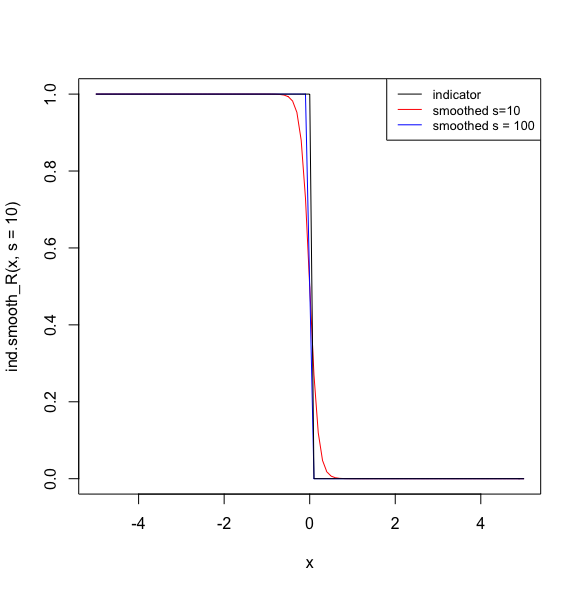
\includegraphics[width=0.5\textwidth]{smoothfun.png}
\caption{Smooth function for indicator function $\mathfrak 1(x\leq 0)$.}
\label{fig:smoothfun}
\end{figure}

Specifically, we use
\begin{equation}\label{eq:indsmooth}
  S_{ij}(\bm \theta;s) := S(e_i(\bm \theta)-e_j(\bm \theta);s)
  = \frac{1}{1+\exp(s\cdot(e_i(\bm \theta)-e_j(\bm \theta)))}.
\end{equation}
Notice that as long as \(e_i(\bm \theta)\) is a continuous function of \(\bm \theta\) for all \(i=1,\cdots,n\), then (\ref{eq:indsmooth}) is indeed a continuous function of \(\bm \theta\).

The log smoothed censored EL (log SCEL) is then defined as
\begin{equation}\label{eq:logel_smoo}
  \ell_{\textrm{SCEL}}(\bm \theta) = \sum_{i=1}^n \Bigl[\delta_i\log(w_i(\bm \theta)) +
    (1-\delta_i)\log(\sum_{j=1}^n S_{ij}(\bm \theta;s)\cdot w_j(\bm \theta))\Bigr].
\end{equation}

\hypertarget{software-design-and-illustrations}{%
\section{Software Design and Illustrations}\label{software-design-and-illustrations}}

The core functionality of \pkg{flexEL} is to support fast and flexible computation of empirical likelihood given estimating equations. The package also supports regression with right-censored responses based on an EM algorithm described in the previous section. Other utilities include support correction and continuity correction which are easily turned on and off by the users.

The package's source code is written as a header-only library in C++ using object-oriented programming. The main class \texttt{GenEL} provides the core computations of weighted log empirical likelihood. \texttt{CensEL} class utilizes \texttt{GenEL} and contains the EM algorithm for right-censored EL computations. The package also provides an \proglang{R} interface mimicking the class structure in C++ based on R6. An R6 object created via the \proglang{R} interface connects to the C++ layer with an external pointer. In this way, fast computation and efficient memory allocation can be achieved. This section describes how a user can interact with the package either in C++ or \proglang{R}.

In terms of built-in models, \pkg{flexEL} provides implementations of estimating equations for mean and quantile regressions based on the following location-scale model:

\begin{equation} \label{md:lsmod}
  y_i = \bm x_i'\bm \beta+ \sigma\cdot\exp(\bm z_i'\bm \gamma)\cdot\varepsilon_i, \quad i=1,\cdots,n,
\end{equation}

as well as the common location model:

\begin{equation} \label{md:lmod}
  y_i = \bm x_i'\bm \beta+ \varepsilon_i, \quad i=1,\cdots,n.
\end{equation}

Users can also leverage the EL calculation for customized models specified by estimating equations, in which case, a user can either create a function in \proglang{R} that returns the \texttt{G} matrix given the value of the parameters (call it e.g.~\texttt{evalG}), or implement the calculation in C++ before wrapping into an \proglang{R} interface.

Several optimization routines are available in \proglang{R}. If analytic gradient of \texttt{G} with respect to the parameters can be derived, a user can also provide a corresponding gradient function. Combined with the gradient of log EL with respect to \texttt{G} via chain rule, a user can then utilize \texttt{optim} or \texttt{nlm} in \proglang{R} for parameter estimation with gradient-based methods.

\hypertarget{mean-regression}{%
\subsection{Mean Regression}\label{mean-regression}}

In this section, we illustrate how one can interact with the C++ API or \proglang{R} API with the built-in location mean regression model and achieve parameter estimation in \proglang{R}.

The following script creates a function in C++ that can be exported to \proglang{R} using Rcpp:

\begin{Shaded}
\begin{Highlighting}[]
\CommentTok{// [[Rcpp::depends("flexEL")]]}
\CommentTok{// [[Rcpp::depends("RcppEigen")]]}

\PreprocessorTok{\#include }\ImportTok{\textless{}Rcpp.h\textgreater{}}
\PreprocessorTok{\#include }\ImportTok{\textless{}RcppEigen.h\textgreater{}}
\PreprocessorTok{\#include }\ImportTok{\textless{}flexEL/gen\_el.h\textgreater{}}
\PreprocessorTok{\#include }\ImportTok{\textless{}flexEL/mean\_reg\_model.h\textgreater{}}

\CommentTok{// [[Rcpp::export]]}
\DataTypeTok{double}\NormalTok{ mr\_neglogel(Eigen::VectorXd beta,}
\NormalTok{                   Eigen::VectorXd y,}
\NormalTok{                   Eigen::MatrixXd X,}
                   \DataTypeTok{bool}\NormalTok{ verbose) \{}
\NormalTok{  flexEL::MeanRegModel MR(y, X); }\CommentTok{// initiate MeanRegModel object with data}
  \DataTypeTok{int}\NormalTok{ n\_obs = MR.get\_n\_obs();}
  \DataTypeTok{int}\NormalTok{ n\_eqs = MR.get\_n\_eqs();}
\NormalTok{  MatrixXd G = MatrixXd::Zero(n\_eqs, n\_obs);}
\NormalTok{  MR.eval\_G(G, beta); }\CommentTok{// obtain G matrix given certain parameter values}
\NormalTok{  flexEL::GenEL GEL(n\_obs, n\_eqs); }\CommentTok{// initiate GenEL object given dimensions}
\NormalTok{  GEL.set\_supp\_adj(true); }\CommentTok{// turn on support correction}
  \DataTypeTok{double}\NormalTok{ logel = GEL.logel(G); }\CommentTok{// obtain log EL}
  \ControlFlowTok{if}\NormalTok{(verbose) \{}
    \DataTypeTok{int}\NormalTok{ n\_iter;}
    \DataTypeTok{double}\NormalTok{ max\_err;}
\NormalTok{    GEL.get\_diag(n\_iter, max\_err); }\CommentTok{// get diagnostics}
\NormalTok{    Rprintf(}\StringTok{"n\_iter = \%i, max\_err = \%f}\SpecialCharTok{\textbackslash{}n}\StringTok{"}\NormalTok{, n\_iter, max\_err);}
\NormalTok{  \}}
  \ControlFlowTok{return}\NormalTok{({-}logel);}
\NormalTok{\}}
\end{Highlighting}
\end{Shaded}

After sourcing the function into \proglang{R} with Rcpp, one can then use e.g.~\texttt{nlm} for negative log EL minimization. The following uses simulated data to illustrate this:

\begin{Shaded}
\begin{Highlighting}[]
\NormalTok{R}\SpecialCharTok{\textgreater{}}\NormalTok{ Rcpp}\SpecialCharTok{::}\FunctionTok{sourceCpp}\NormalTok{(}\StringTok{"mr\_neglogel.cpp"}\NormalTok{)}
\NormalTok{R}\SpecialCharTok{\textgreater{}}\NormalTok{ beta0 }\OtherTok{\textless{}{-}} \FunctionTok{c}\NormalTok{(}\DecValTok{1}\NormalTok{,}\DecValTok{2}\NormalTok{)}
\NormalTok{R}\SpecialCharTok{\textgreater{}}\NormalTok{ n }\OtherTok{\textless{}{-}} \DecValTok{200}
\NormalTok{R}\SpecialCharTok{\textgreater{}}\NormalTok{ X }\OtherTok{\textless{}{-}} \FunctionTok{cbind}\NormalTok{(}\DecValTok{1}\NormalTok{, }\FunctionTok{rnorm}\NormalTok{(n))}
\NormalTok{R}\SpecialCharTok{\textgreater{}}\NormalTok{ eps }\OtherTok{\textless{}{-}} \FunctionTok{rnorm}\NormalTok{(n)}
\NormalTok{R}\SpecialCharTok{\textgreater{}}\NormalTok{ y }\OtherTok{\textless{}{-}} \FunctionTok{c}\NormalTok{(X }\SpecialCharTok{\%*\%}\NormalTok{ beta0 }\SpecialCharTok{+}\NormalTok{ eps)}
\NormalTok{R}\SpecialCharTok{\textgreater{}} \CommentTok{\# mr\_neglogel(c(0.75, 1.25), t(X), y, verbose = TRUE)}
\NormalTok{R}\SpecialCharTok{\textgreater{}} \FunctionTok{nlm}\NormalTok{(mr\_neglogel, }\FunctionTok{c}\NormalTok{(}\FloatTok{0.75}\NormalTok{, }\FloatTok{1.25}\NormalTok{), y, }\FunctionTok{t}\NormalTok{(X), }\ConstantTok{FALSE}\NormalTok{)}
\end{Highlighting}
\end{Shaded}

\begin{verbatim}
$minimum
[1] 1065.964

$estimate
[1] 1.102879 2.086755

$gradient
[1] 3.092455e-05 1.612614e-05

$code
[1] 1

$iterations
[1] 7
\end{verbatim}

If a user wishes not to use the C++ API directly, they can write a similar function in \proglang{R} as follows:

\begin{Shaded}
\begin{Highlighting}[]
\NormalTok{R}\SpecialCharTok{\textgreater{}} \FunctionTok{library}\NormalTok{(flexEL)}
\NormalTok{R}\SpecialCharTok{\textgreater{}}\NormalTok{ mr\_neglogel }\OtherTok{\textless{}{-}} \ControlFlowTok{function}\NormalTok{(beta, y, X, gel) \{}
\SpecialCharTok{+}\NormalTok{    G }\OtherTok{\textless{}{-}}\NormalTok{ flexEL}\SpecialCharTok{::}\FunctionTok{mr\_evalG}\NormalTok{(y, X, beta)}
\SpecialCharTok{+}    \FunctionTok{return}\NormalTok{(}\SpecialCharTok{{-}}\NormalTok{gel}\SpecialCharTok{$}\FunctionTok{logel}\NormalTok{(G))}
\SpecialCharTok{+}\NormalTok{  \}}
\NormalTok{R}\SpecialCharTok{\textgreater{}} 
\NormalTok{R}\SpecialCharTok{\textgreater{}}\NormalTok{ gel }\OtherTok{\textless{}{-}}\NormalTok{ flexEL}\SpecialCharTok{::}\NormalTok{GenEL}\SpecialCharTok{$}\FunctionTok{new}\NormalTok{(}\AttributeTok{n\_obs =}\NormalTok{ n, }\AttributeTok{n\_eqs =} \DecValTok{2}\NormalTok{) }\CommentTok{\# initalize an GenEL object}
\NormalTok{R}\SpecialCharTok{\textgreater{}}\NormalTok{ gel}\SpecialCharTok{$}\NormalTok{supp\_adj }\OtherTok{\textless{}{-}} \ConstantTok{TRUE} \CommentTok{\# turn on support correction}
\NormalTok{R}\SpecialCharTok{\textgreater{}} 
\NormalTok{R}\SpecialCharTok{\textgreater{}} \FunctionTok{nlm}\NormalTok{(mr\_neglogel, }\FunctionTok{c}\NormalTok{(}\FloatTok{0.75}\NormalTok{, }\FloatTok{1.25}\NormalTok{), y, X, gel)}
\end{Highlighting}
\end{Shaded}

\begin{verbatim}
$minimum
[1] 1065.964

$estimate
[1] 1.102879 2.086755

$gradient
[1] 3.092455e-05 1.612614e-05

$code
[1] 1

$iterations
[1] 7
\end{verbatim}

The usage is similar with right-censored outcomes, e.g.~using \proglang{R}:

\begin{Shaded}
\begin{Highlighting}[]
\NormalTok{R}\SpecialCharTok{\textgreater{}}\NormalTok{ mr\_neglogcel }\OtherTok{\textless{}{-}} \ControlFlowTok{function}\NormalTok{(beta, y\_obs, X, cel) \{}
\SpecialCharTok{+}\NormalTok{    G }\OtherTok{\textless{}{-}}\NormalTok{ flexEL}\SpecialCharTok{::}\FunctionTok{mr\_evalG}\NormalTok{(y, X, beta)}
\SpecialCharTok{+}    \SpecialCharTok{{-}}\NormalTok{gel}\SpecialCharTok{$}\FunctionTok{logel}\NormalTok{(G)}
\SpecialCharTok{+}\NormalTok{  \}}
\NormalTok{R}\SpecialCharTok{\textgreater{}} 
\NormalTok{R}\SpecialCharTok{\textgreater{}}\NormalTok{ cel }\OtherTok{\textless{}{-}}\NormalTok{ flexEL}\SpecialCharTok{::}\NormalTok{CensEL}\SpecialCharTok{$}\FunctionTok{new}\NormalTok{(}\AttributeTok{n\_obs =}\NormalTok{ n, }\AttributeTok{n\_eqs =} \DecValTok{2}\NormalTok{)}
\NormalTok{R}\SpecialCharTok{\textgreater{}}\NormalTok{ cel}\SpecialCharTok{$}\NormalTok{supp\_adj }\OtherTok{\textless{}{-}} \ConstantTok{TRUE}
\NormalTok{R}\SpecialCharTok{\textgreater{}}\NormalTok{ cel}\SpecialCharTok{$}\NormalTok{smooth }\OtherTok{\textless{}{-}} \ConstantTok{TRUE} \CommentTok{\# turn on continuity correction}
\NormalTok{R}\SpecialCharTok{\textgreater{}}\NormalTok{ cel}\SpecialCharTok{$}\NormalTok{smooth\_s }\OtherTok{\textless{}{-}} \DecValTok{1} \CommentTok{\# set tuning parameter for continuity correction}
\NormalTok{R}\SpecialCharTok{\textgreater{}} 
\NormalTok{R}\SpecialCharTok{\textgreater{}}\NormalTok{ z }\OtherTok{\textless{}{-}} \FunctionTok{rnorm}\NormalTok{(}\DecValTok{2}\SpecialCharTok{*}\FunctionTok{mean}\NormalTok{(y), }\AttributeTok{n =}\NormalTok{ n) }\CommentTok{\# censoring variable}
\NormalTok{R}\SpecialCharTok{\textgreater{}}\NormalTok{ delta }\OtherTok{\textless{}{-}}\NormalTok{ y }\SpecialCharTok{\textless{}=}\NormalTok{ z }\CommentTok{\# censoring indicators}
\NormalTok{R}\SpecialCharTok{\textgreater{}}\NormalTok{ y\_obs }\OtherTok{\textless{}{-}}\NormalTok{ y}
\NormalTok{R}\SpecialCharTok{\textgreater{}}\NormalTok{ y\_obs[}\SpecialCharTok{!}\NormalTok{delta] }\OtherTok{\textless{}{-}}\NormalTok{ z[}\SpecialCharTok{!}\NormalTok{delta]}
\NormalTok{R}\SpecialCharTok{\textgreater{}} 
\NormalTok{R}\SpecialCharTok{\textgreater{}} \FunctionTok{nlm}\NormalTok{(mr\_neglogcel, }\FunctionTok{c}\NormalTok{(}\FloatTok{0.75}\NormalTok{, }\FloatTok{1.25}\NormalTok{), y\_obs, X, cel)}
\end{Highlighting}
\end{Shaded}

\begin{verbatim}
$minimum
[1] 1065.964

$estimate
[1] 1.102879 2.086755

$gradient
[1] 3.092455e-05 1.612614e-05

$code
[1] 1

$iterations
[1] 7
\end{verbatim}

\hypertarget{quantile-regression}{%
\subsection{Quantile Regression}\label{quantile-regression}}

For the location-scale model \eqref{md:lsmod}, the \(\tau\times 100\%\) conditional quantile of \(y_i\) is
\begin{equation} \label{eq:lsqr}
  Q_{\tau}(y_i|\bm x_i) = \bm x_i' \bm \beta+ \sigma\cdot\exp(\bm z_i' \bm \gamma)\cdot\nu_{\tau}.
\end{equation}

In this case, for parameters \(\bm \beta,\bm \gamma\) and \(\sigma\), we adopt the same estimating equation as in the mean regression case. For the quantile parameter \(\nu_{\tau}\), we rely on the ``check function'' introduced by Koenker and Bassett Jr (1978), which is defined as
\begin{equation}\label{eq:check}
\rho_\tau(u) = u\cdot(\tau - \mathfrak 1 \{u \le 0\}),
\end{equation}
where \(\mathfrak 1\{\cdot\}\) is the indicator function.

If the \(\tau\)-th quantile value of \(\varepsilon_i\stackrel {\textrm{iid}}{\sim}(0,1)\) is \(\nu_{\tau}\), then \(\varepsilon_i-\nu_{\tau}\) has \(\tau\)-th quantile value \(0\). The estimator of \(\nu_{\tau}\) is then defined as
\begin{equation}\label{eq:nueq}
  \hat\nu_{\tau} = \mathop{\mathrm{arg\,min}}_{\tilde\nu_{\tau}} \textrm{E}\Biggl[\rho_{\tau}\Bigl(\frac{y-\bm x'\bm \beta}{\sigma\cdot\exp(\bm z'\gamma)}-\tilde\nu_{\tau}\Bigr)\Biggr].
\end{equation}

As before, we use the first order optimality condition of (\ref{eq:nueq}) to obtain the estimating equation for \(\nu_{\tau}\). Therefore, we obtain all the moment conditions for quantile regression as follows
\begin{equation} \label{eq:qrls}
\begin{split}
  \textrm{E}\Bigl[\frac{y-\bm x'\bm \beta}{\exp(2\bm z'\bm \gamma)}\cdot\bm x\Bigr] &= 0 \\
  \textrm{E}\Bigl[\bigl(1-\frac{(y-\bm x'\bm \beta)^2}{\sigma^2\cdot\exp(2\bm z'\bm \gamma)}\bigr)\cdot\bm z\Bigr] &= 0 \\
  \textrm{E}\Bigl[\frac{(y-\bm x'\bm \beta)^2}{\sigma^2\cdot\exp(2\bm z'\bm \gamma)}-1\Bigr] &= 0 \\
  \textrm{E}\Bigl[\rho'_{\tau}\bigl(\frac{y-\bm x'\bm \beta}{\sigma\cdot\exp(\bm z'\bm \gamma)}-\nu_{\tau}\bigr)\Bigr] &= 0.
\end{split}
\end{equation}

Notice that the indicator function used by the ``check function'' is also a source of discontinuity in log EL even in the absence of censoring. Although there are other approaches to smooth out the discontinuity in quantile regression, such as C. Chen (2007), splines or kernel methods, the same trick used for correcting the discontinuity caused by right-censoring is particularly straightforward to apply here as well. That is, we modify \eqref{eq:check} as follows:

\begin{equation}
\rho_{S,\tau}(u;s) = u\cdot(\tau - S(u;s)),
\end{equation}
where \(S\) is defined as in \eqref{eq:sigmoid}.

Usage of quantile regression in \pkg{flexEL} is very similar to mean regression in the last section. Moreover, one can simultaneously estimte parameters at multiple quantile levels both with the location and location-scale models. With the location model, both the intercept and the slope parameters can be different at different quantile levels. Essentially, the \texttt{G} matrix is obtained by stacking together multiple \texttt{G} matrices each at one quantile level. This is one advantage of quantile regression when heteroscedasticity presents. With the location-scale model, only the quantile parameter \(\nu_{\tau}\) is different at different quantile levels, since heteroscedasticity can be handled by the scale function.

\hypertarget{user-defined-model}{%
\subsection{User-defined Model}\label{user-defined-model}}

The following toy example illustrates how to use \pkg{flexEL} with a customized model. Consider a simple two-parameter linear regression model
\[
  y_i = \beta_0 + \beta_1x_i + \varepsilon_i, \quad i=1,\cdots,n, 
\]
where \(\epsilon_i \stackrel {\textrm{iid}}{\sim}\text{F}(\epsilon)\) such that \(\textrm{E}(\epsilon_i) = 0\) and \(\text{Var}(\epsilon_i) = 1\).

As the first step, one should design the estimating equations of the parameters and implement a function (\texttt{evalG}) that returns the corresponding \(G\) matrix of dimension \(n\times m\), where \(n\) is the number of observations, and \(m\) is the dimension of the range of the estimating equation.

In this example, the following estimating equation can be used, which has a range of dimension \(m=p\), same as the dimension of the parameter vector \(\beta\):
\[
  \textrm{E}[(y-x'\beta)\cdot x] = 0,
\]
which is
\[
  \sum_{i=1}^n w_i\cdot (y_i-x_i'\beta)\cdot x_i = 0.
\]
In other words, the \(g\) function is specified as
\[
  g(x,y;\beta) = (y-x'\beta)\cdot x.
\]

This can be implemented in R (called \texttt{mr2\_evalG}) as follows:

\begin{Shaded}
\begin{Highlighting}[]
\NormalTok{R}\SpecialCharTok{\textgreater{}}\NormalTok{ mr2\_evalG }\OtherTok{\textless{}{-}} \ControlFlowTok{function}\NormalTok{(y, X, beta) \{}
\SpecialCharTok{+}\NormalTok{    tX }\OtherTok{\textless{}{-}} \FunctionTok{t}\NormalTok{(X)}
\SpecialCharTok{+}\NormalTok{    yXb }\OtherTok{\textless{}{-}}\NormalTok{ y }\SpecialCharTok{{-}} \FunctionTok{c}\NormalTok{(X }\SpecialCharTok{\%*\%}\NormalTok{ beta)}
\SpecialCharTok{+}\NormalTok{    G }\OtherTok{\textless{}{-}} \FunctionTok{sweep}\NormalTok{(tX, }\AttributeTok{MARGIN =} \DecValTok{2}\NormalTok{, yXb, }\StringTok{\textasciigrave{}}\AttributeTok{*}\StringTok{\textasciigrave{}}\NormalTok{)}
\SpecialCharTok{+}    \FunctionTok{return}\NormalTok{(}\FunctionTok{t}\NormalTok{(G))}
\SpecialCharTok{+}\NormalTok{  \}}
\end{Highlighting}
\end{Shaded}

With \pkg{flexEL}, the negative log EL can be implemented as:

\begin{Shaded}
\begin{Highlighting}[]
\NormalTok{R}\SpecialCharTok{\textgreater{}}\NormalTok{ mr2\_neglogel }\OtherTok{\textless{}{-}} \ControlFlowTok{function}\NormalTok{(beta, y, X, gel) \{}
\SpecialCharTok{+}\NormalTok{    G }\OtherTok{\textless{}{-}} \FunctionTok{mr2\_evalG}\NormalTok{(y, X, beta)}
\SpecialCharTok{+}    \FunctionTok{return}\NormalTok{(}\SpecialCharTok{{-}}\NormalTok{gel}\SpecialCharTok{$}\FunctionTok{logel}\NormalTok{(G))}
\SpecialCharTok{+}\NormalTok{  \}}
\end{Highlighting}
\end{Shaded}

One may also provide the gradient of \texttt{mr2\_evalG} with respect to the parameters, in this case, it is

\begin{Shaded}
\begin{Highlighting}[]
\NormalTok{R}\SpecialCharTok{\textgreater{}}\NormalTok{ mr2\_dGdb }\OtherTok{\textless{}{-}} \ControlFlowTok{function}\NormalTok{(y, X, beta) \{}
\SpecialCharTok{+}\NormalTok{    lx }\OtherTok{\textless{}{-}} \FunctionTok{split}\NormalTok{(X, }\FunctionTok{row}\NormalTok{(X))}
\SpecialCharTok{+}\NormalTok{    dg }\OtherTok{\textless{}{-}} \FunctionTok{lapply}\NormalTok{(lx, }\ControlFlowTok{function}\NormalTok{(x) }\SpecialCharTok{{-}}\FunctionTok{tcrossprod}\NormalTok{(x,x))}
\SpecialCharTok{+}    \FunctionTok{return}\NormalTok{(dg)}
\SpecialCharTok{+}\NormalTok{  \}}
\end{Highlighting}
\end{Shaded}

Notice that here the gradient is a 3-dimensional matrix. This can then be combined with the gradient of log EL w.r.t \texttt{G} to obtain the gradient of log EL w.r.t. the parameters, \(\beta\):

\begin{Shaded}
\begin{Highlighting}[]
\NormalTok{R}\SpecialCharTok{\textgreater{}}\NormalTok{ mr2\_neglogel\_grad }\OtherTok{\textless{}{-}} \ControlFlowTok{function}\NormalTok{(beta, y, X, gel) \{}
\SpecialCharTok{+}\NormalTok{    G }\OtherTok{\textless{}{-}} \FunctionTok{mr2\_evalG}\NormalTok{(y, X, beta)}
\SpecialCharTok{+}\NormalTok{    logel\_lst }\OtherTok{\textless{}{-}}\NormalTok{ gel}\SpecialCharTok{$}\FunctionTok{logel\_grad}\NormalTok{(G)}
\SpecialCharTok{+}\NormalTok{    dldG }\OtherTok{\textless{}{-}} \SpecialCharTok{{-}}\NormalTok{logel\_lst}\SpecialCharTok{$}\NormalTok{dldG}
\SpecialCharTok{+}\NormalTok{    dGdb }\OtherTok{\textless{}{-}} \FunctionTok{mr2\_dGdb}\NormalTok{(y, X, beta)}
\SpecialCharTok{+}\NormalTok{    grad\_mat }\OtherTok{\textless{}{-}} \FunctionTok{matrix}\NormalTok{(}\ConstantTok{NA}\NormalTok{, }\AttributeTok{nrow =} \FunctionTok{nrow}\NormalTok{(dldG), }\AttributeTok{ncol =} \FunctionTok{ncol}\NormalTok{(dldG))}
\SpecialCharTok{+}    \ControlFlowTok{for}\NormalTok{ (ii }\ControlFlowTok{in} \DecValTok{1}\SpecialCharTok{:}\FunctionTok{nrow}\NormalTok{(dldG)) \{}
\SpecialCharTok{+}\NormalTok{      grad\_mat[ii,] }\OtherTok{\textless{}{-}}\NormalTok{ dGdb[[ii]] }\SpecialCharTok{\%*\%}\NormalTok{ dldG[ii,]}
\SpecialCharTok{+}\NormalTok{    \}}
\SpecialCharTok{+}    \FunctionTok{colSums}\NormalTok{(grad\_mat)}
\SpecialCharTok{+}\NormalTok{  \}}
\end{Highlighting}
\end{Shaded}

Then one can use e.g.~\texttt{optim} to obtain the estimate of \(\beta\):

\begin{Shaded}
\begin{Highlighting}[]
\NormalTok{R}\SpecialCharTok{\textgreater{}} \FunctionTok{library}\NormalTok{(flexEL)}
\NormalTok{R}\SpecialCharTok{\textgreater{}} 
\NormalTok{R}\SpecialCharTok{\textgreater{}} \CommentTok{\# simulate some data}
\NormalTok{R}\SpecialCharTok{\textgreater{}}\NormalTok{ n }\OtherTok{\textless{}{-}} \DecValTok{200}
\NormalTok{R}\SpecialCharTok{\textgreater{}}\NormalTok{ X }\OtherTok{\textless{}{-}} \FunctionTok{cbind}\NormalTok{(}\DecValTok{1}\NormalTok{, }\FunctionTok{rnorm}\NormalTok{(n))}
\NormalTok{R}\SpecialCharTok{\textgreater{}}\NormalTok{ beta0 }\OtherTok{\textless{}{-}} \FunctionTok{c}\NormalTok{(}\DecValTok{1}\NormalTok{, }\DecValTok{2}\NormalTok{)}
\NormalTok{R}\SpecialCharTok{\textgreater{}}\NormalTok{ eps }\OtherTok{\textless{}{-}}\NormalTok{ (}\FunctionTok{rchisq}\NormalTok{(n, }\AttributeTok{df=}\DecValTok{5}\NormalTok{)}\SpecialCharTok{{-}}\DecValTok{5}\NormalTok{)}\SpecialCharTok{/}\FunctionTok{sqrt}\NormalTok{(}\DecValTok{2}\SpecialCharTok{*}\DecValTok{5}\NormalTok{)}
\NormalTok{R}\SpecialCharTok{\textgreater{}}\NormalTok{ y }\OtherTok{\textless{}{-}} \FunctionTok{c}\NormalTok{(X }\SpecialCharTok{\%*\%}\NormalTok{ beta0) }\SpecialCharTok{+}\NormalTok{ eps}
\NormalTok{R}\SpecialCharTok{\textgreater{}} 
\NormalTok{R}\SpecialCharTok{\textgreater{}}\NormalTok{ gel }\OtherTok{\textless{}{-}}\NormalTok{ GenEL}\SpecialCharTok{$}\FunctionTok{new}\NormalTok{(}\AttributeTok{n\_obs =}\NormalTok{ n, }\AttributeTok{n\_eqs =} \DecValTok{2}\NormalTok{)}
\NormalTok{R}\SpecialCharTok{\textgreater{}}\NormalTok{ gel}\SpecialCharTok{$}\NormalTok{supp\_adj }\OtherTok{\textless{}{-}} \ConstantTok{TRUE}
\NormalTok{R}\SpecialCharTok{\textgreater{}} 
\NormalTok{R}\SpecialCharTok{\textgreater{}} \FunctionTok{optim}\NormalTok{(}\FunctionTok{c}\NormalTok{(}\FloatTok{0.75}\NormalTok{, }\FloatTok{1.25}\NormalTok{), }\AttributeTok{fn =}\NormalTok{ mr2\_neglogel, }\AttributeTok{gr =}\NormalTok{ mr2\_neglogel\_grad,}
\SpecialCharTok{+}\NormalTok{        y, X, gel, }\AttributeTok{method =} \StringTok{"BFGS"}\NormalTok{)}
\end{Highlighting}
\end{Shaded}

\begin{verbatim}
$par
[1] 0.9289329 2.0070245

$value
[1] 1065.964

$counts
function gradient 
      32       10 

$convergence
[1] 0

$message
NULL
\end{verbatim}

Alternatively, a user can implement the \texttt{G} matrix and gradient calculations in C++ and follows the example in the mean regression section where instead of including \texttt{flexEL/mean\_reg\_model.h}, include the user defined C++ header file.

\hypertarget{bayesian-el}{%
\subsection{Bayesian EL}\label{bayesian-el}}

\begin{itemize}
\item
  Good to illustrate with \proglang{Stan} NUTS algorithm, because we've implemented it already and \proglang{Stan} is a really good autodiff engine + best NUTS implementation.
\item
  Can illustrate with the example from the JRSSB EL-HMC paper.
\end{itemize}

\hypertarget{conclusion}{%
\section*{Conclusion}\label{conclusion}}
\addcontentsline{toc}{section}{Conclusion}

\hypertarget{refs}{}
\begin{CSLReferences}{1}{0}
\leavevmode\hypertarget{ref-chaudhuri-et-al2017}{}%
Chaudhuri, Sanjay, Debashis Mondal, and Teng Yin. 2017. {``Hamiltonian Monte Carlo Sampling in Bayesian Empirical Likelihood Computation.''} \emph{Journal of the Royal Statistical Society: Series B (Statistical Methodology)} 79 (1): 293--320.

\leavevmode\hypertarget{ref-chen2007}{}%
Chen, Colin. 2007. {``A Finite Smoothing Algorithm for Quantile Regression.''} \emph{Journal of Computational and Graphical Statistics} 16 (1): 136--64.

\leavevmode\hypertarget{ref-chen-et-al2008}{}%
Chen, Jiahua, Asokan Mulayath Variyath, and Bovas Abraham. 2008. {``Adjusted Empirical Likelihood and Its Properties.''} \emph{Journal of Computational and Graphical Statistics} 17 (2): 426--43.

\leavevmode\hypertarget{ref-efron1981}{}%
Efron, Bradley. 1981. {``Nonparametric Standard Errors and Confidence Intervals.''} \emph{Canadian Journal of Statistics} 9 (2): 139--58.

\leavevmode\hypertarget{ref-he-et-al2016}{}%
He, Shuyuan, Wei Liang, Junshan Shen, and Grace Yang. 2016. {``Empirical Likelihood for Right Censored Lifetime Data.''} \emph{Journal of the American Statistical Association} 111 (514): 646--55.

\leavevmode\hypertarget{ref-koenker-bassett1978}{}%
Koenker, Roger, and Gilbert Bassett Jr. 1978. {``Regression Quantiles.''} \emph{Econometrica: Journal of the Econometric Society}, 33--50.

\leavevmode\hypertarget{ref-kolaczyk1994}{}%
Kolaczyk, Eric D. 1994. {``Empirical Likelihood for Generalized Linear Models.''} \emph{Statistica Sinica}, 199--218.

\leavevmode\hypertarget{ref-lazar2003}{}%
Lazar, Nicole A. 2003. {``Bayesian Empirical Likelihood.''} \emph{Biometrika} 90 (2): 319--26.

\leavevmode\hypertarget{ref-li-wang2003}{}%
Li, Gang, and Qi-Hua Wang. 2003. {``Empirical Likelihood Regression Analysis for Right Censored Data.''} \emph{Statistica Sinica}, 51--68.

\leavevmode\hypertarget{ref-newey-smith2004}{}%
Newey, Whitney K, and Richard J Smith. 2004. {``Higher Order Properties of GMM and Generalized Empirical Likelihood Estimators.''} \emph{Econometrica} 72 (1): 219--55.

\leavevmode\hypertarget{ref-ning-et-al2013}{}%
Ning, J, J Qin, M Asgharian, and Y Shen. 2013. {``Empirical Likelihood-Based Confidence Intervals for Length-Biased Data.''} \emph{Statistics in Medicine} 32 (13): 2278--91.

\leavevmode\hypertarget{ref-owen1988}{}%
Owen, Art. 1988. {``Empirical Likelihood Ratio Confidence Intervals for a Single Functional.''} \emph{Biometrika} 75 (2): 237--49.

\leavevmode\hypertarget{ref-owen1990}{}%
---------. 1990. {``Empirical Likelihood Ratio Confidence Regions.''} \emph{The Annals of Statistics}, 90--120.

\leavevmode\hypertarget{ref-owen1991}{}%
---------. 1991. {``Empirical Likelihood for Linear Models.''} \emph{The Annals of Statistics}, 1725--47.

\leavevmode\hypertarget{ref-qin-lawless1994}{}%
Qin, Jin, and Jerry Lawless. 1994. {``Empirical Likelihood and General Estimating Equations.''} \emph{The Annals of Statistics}, 300--325.

\leavevmode\hypertarget{ref-schennach2005}{}%
Schennach, Susanne M. 2005. {``Bayesian Exponentially Tilted Empirical Likelihood.''} \emph{Biometrika} 92 (1): 31--46.

\leavevmode\hypertarget{ref-schennach2007}{}%
---------. 2007. {``Point Estimation with Exponentially Tilted Empirical Likelihood.''} \emph{The Annals of Statistics}, 634--72.

\leavevmode\hypertarget{ref-shen-et-al2016}{}%
Shen, Junshan, Kam Chuen Yuen, and Chunling Liu. 2016. {``Empirical Likelihood Confidence Regions for One-or Two-Samples with Doubly Censored Data.''} \emph{Computational Statistics \& Data Analysis} 93: 285--93.

\leavevmode\hypertarget{ref-thomas-grunkemeier1975}{}%
Thomas, David R, and Gary L Grunkemeier. 1975. {``Confidence Interval Estimation of Survival Probabilities for Censored Data.''} \emph{Journal of the American Statistical Association} 70 (352): 865--71.

\leavevmode\hypertarget{ref-zhou2005}{}%
Zhou, Mai. 2005. {``Empirical Likelihood Ratio with Arbitrarily Censored/Truncated Data by EM Algorithm.''} \emph{Journal of Computational and Graphical Statistics} 14 (3): 643--56.

\leavevmode\hypertarget{ref-zhou-et-al2012}{}%
Zhou, Mai, Mi-Ok Kim, and Arne C Bathke. 2012. {``Empirical Likelihood Analysis for the Heteroscedastic Accelerated Failure Time Model.''} \emph{Statistica Sinica}, 295--316.

\leavevmode\hypertarget{ref-zhou-li2008}{}%
Zhou, Mai, and Gang Li. 2008. {``Empirical Likelihood Analysis of the Buckley--James Estimator.''} \emph{Journal of Multivariate Analysis} 99 (4): 649--64.

\end{CSLReferences}

\end{document}
